%%%%%%%%%%%%%%%%%%
% simPH package vignette
% Christopher Gandrud
% 15 May 2013
%%%%%%%%%%%%%%%%%%


\documentclass[nojss]{jss}\usepackage{graphicx, color}
%% maxwidth is the original width if it is less than linewidth
%% otherwise use linewidth (to make sure the graphics do not exceed the margin)
\makeatletter
\def\maxwidth{ %
  \ifdim\Gin@nat@width>\linewidth
    \linewidth
  \else
    \Gin@nat@width
  \fi
}
\makeatother

\definecolor{fgcolor}{rgb}{0.2, 0.2, 0.2}
\newcommand{\hlnumber}[1]{\textcolor[rgb]{0,0,0}{#1}}%
\newcommand{\hlfunctioncall}[1]{\textcolor[rgb]{0.501960784313725,0,0.329411764705882}{\textbf{#1}}}%
\newcommand{\hlstring}[1]{\textcolor[rgb]{0.6,0.6,1}{#1}}%
\newcommand{\hlkeyword}[1]{\textcolor[rgb]{0,0,0}{\textbf{#1}}}%
\newcommand{\hlargument}[1]{\textcolor[rgb]{0.690196078431373,0.250980392156863,0.0196078431372549}{#1}}%
\newcommand{\hlcomment}[1]{\textcolor[rgb]{0.180392156862745,0.6,0.341176470588235}{#1}}%
\newcommand{\hlroxygencomment}[1]{\textcolor[rgb]{0.43921568627451,0.47843137254902,0.701960784313725}{#1}}%
\newcommand{\hlformalargs}[1]{\textcolor[rgb]{0.690196078431373,0.250980392156863,0.0196078431372549}{#1}}%
\newcommand{\hleqformalargs}[1]{\textcolor[rgb]{0.690196078431373,0.250980392156863,0.0196078431372549}{#1}}%
\newcommand{\hlassignement}[1]{\textcolor[rgb]{0,0,0}{\textbf{#1}}}%
\newcommand{\hlpackage}[1]{\textcolor[rgb]{0.588235294117647,0.709803921568627,0.145098039215686}{#1}}%
\newcommand{\hlslot}[1]{\textit{#1}}%
\newcommand{\hlsymbol}[1]{\textcolor[rgb]{0,0,0}{#1}}%
\newcommand{\hlprompt}[1]{\textcolor[rgb]{0.2,0.2,0.2}{#1}}%

\usepackage{framed}
\makeatletter
\newenvironment{kframe}{%
 \def\at@end@of@kframe{}%
 \ifinner\ifhmode%
  \def\at@end@of@kframe{\end{minipage}}%
  \begin{minipage}{\columnwidth}%
 \fi\fi%
 \def\FrameCommand##1{\hskip\@totalleftmargin \hskip-\fboxsep
 \colorbox{shadecolor}{##1}\hskip-\fboxsep
     % There is no \\@totalrightmargin, so:
     \hskip-\linewidth \hskip-\@totalleftmargin \hskip\columnwidth}%
 \MakeFramed {\advance\hsize-\width
   \@totalleftmargin\z@ \linewidth\hsize
   \@setminipage}}%
 {\par\unskip\endMakeFramed%
 \at@end@of@kframe}
\makeatother

\definecolor{shadecolor}{rgb}{.97, .97, .97}
\definecolor{messagecolor}{rgb}{0, 0, 0}
\definecolor{warningcolor}{rgb}{1, 0, 1}
\definecolor{errorcolor}{rgb}{1, 0, 0}
\newenvironment{knitrout}{}{} % an empty environment to be redefined in TeX

\usepackage{alltt}

\usepackage{amsmath}
\usepackage{graphicx}

%\VignetteEngine{knitr}
%\VignetteIndexEntry{simPH}

%%%% Set up



%%%%%%%%%% Title Page Information 

\title{\pkg{simPH}: Tools for Simulating and Plotting Quantities of Interest from Cox Proportional Hazards Models}
\author{Christopher Ganrud\\Yonsei University}

%%%%%%%% Pretty Print
\Plainauthor{Christopher Gandrud}
\Plaintitle{\pkg{simPH}: Tools for Simulating and Graphing Quantities of Interest from Cox Proportional Hazards Models}
\Shorttitle{\pkg{simPH}: Simulating and Plotting Cox PH Quantities of Interest}

%%%%%% Abstract
\Abstract{
	I describe an \proglang{R} package \pkg{simPH} for simulating and plotting quantities of interest estimated from Cox Proportional Hazards models. The quantities of interest include hazard ratios, relative hazards, first differences, marginal effects, and hazard rates for linear, linear interactive, time-varying, polynomial, and penalized spline estimated effects. The quantities of interest calculated from parameters drawn from the posterior, sampling distribution. The draws are then plotted using a methods that utilize the popular \pkg{ggplot2} package. The package is illustrated using epidemiological and political science data.
}

\Keywords{cox proportional hazards, uncertainty, posterior distribution}

%%%%%%%%%% Address
\Address{
	Christopher Gandrud \\
	Department of International Relations \\
	Yonsei University \\
	208 Jeongui Hall \\
	1 Yonseidae-gil \\
	Wonju, Gangwon-do \\
	220-710, Republic of Korea \\
	E-mail: \email{gandrud@yonsei.ac.kr} \\
	URL: \url{http://christophergandrud.blogspot.com}
}


%%%%%%%% Begin Document
\IfFileExists{upquote.sty}{\usepackage{upquote}}{}
\begin{document}

Results estimated from Cox Proportional Hazards (PH) models are often reported with coefficient point estimates or hazard ratios--exponentiated coefficients--and confidence intervals. However, this approach can (a) obscure the functional form of the estimate, especially over time and when it is non-linear or interactive and (b) give an inadequate sense of the uncertainty surrounding the estimates. There are currently limited capabilities in \proglang{R}\footnote{The \pkg{survival} \citep{R-survival} and \pkg{Zelig} \citep{R-Zelig} packages do included limited functions for presenting estimates from Cox PH models with uncertainty. However, they have very limited or nonexistent capabilities to show nonlinear and interactive estimates with associated uncertainty.} and popular statistical software such as Stata to present results in any other way. The \pkg{simPH} \citep{R-simPH} \proglang{R} package aims to make it much easier for researchers to show their Cox PH results. 

Drawing directly from approaches taken by \cite{King2000} and \cite{Licht2011} \pkg{simPH} simulates parameter from estimated Cox PH models by drawing them from their posterior distribution. Then it calculates quantities of interests, such as hazard ratios, first differences, relative hazards, marginal effects (for interactions), and hazard ratios. Finally, it plots the distributions of these simulated quantities of interest with visual-weighting \citep{Hsiang2012}. The plots are generally created with the popular \proglang{R} package \pkg{ggplot2} \citep{R-ggplot2} and as such can be aesthetically improved in virtually any way allowed by the package.

In this paper I discuss and provide examples of how to use \pkg{simPH} to simulate and plot quantities of interest estimated from Cox PH models. First, I discuss the quantities of interest \pkg{simPH} calculates and the simulation approach it uses to estimate uncertainty about these quantities. Then I discuss the general steps a researcher takes to use simPH. Finally, give step-by-step instructions for how to use \pkg{simPH} to show results from a variety of quantities of interest for a number of different kinds of estimated covariate relationships including linear, linear interactive, time-varying interactive, polynomial nonlinear, and penalized spline nonlinear. 

\section{Simulating Quantities of Interest}

Results from Cox PH models, and indeed many other methods, are often conveyed using `train-timetables' of coefficient estimates and some measure of uncertainty such as standard errors or confidence intervals. This approach is inadequately informative, especially for effects that are estimated to vary over time, over values of the covariate, or in interaction with other covariates. When researchers do visually communicate uncertainty they often rely on graphical features, such as confidence interval lines that emphasize edges--areas of low likelihood--rather than the center, i.e. estimates that are more strongly supported by the model. The \pkg{simPH} package makes it easy to more fully present results from Cox PH models.


\subsection{Calculating Quantities of Interest}

First let's look at the types of quantities of interest researchers are often interested in estimating from Cox Proportional Hazards models \citep{cox1972}. A basic Cox PH model is given by:
%
\begin{equation}
    h(t|\mathbf{X}_{i}) = h_{0}(t)\mathrm{e}^{(\mathbf{\beta X}_{i})}.
\end{equation}
%
$h(t|\mathbf{X}_{i})$ is the hazard rate for a unit $i$ at time $t$, i.e. the rate at which an event of interest--e.g. cancer remission, a war breaks out--happens. $h_{0}(t)$ is the baseline hazard at time $t$, i.e. the hazard when all covariates are 0. $\mathbf{\beta}$ is a vector of coefficients. $\mathbf{X}_{i}$ is a vector of covariates for unit $i$.

Researchers are often interested in how a given covariate $x$ affects the hazard rate $h(t)$. The simplest approach is to simply report the coefficient $\beta$ for the covariate. It is more common to report the hazard ratio in its simplest form is $\mathrm{e}^{\beta}$. It is a ratio in that it represents the ratio of the hazards of units with two levels of the covariate--all else equal--at a given point in time $(t)$. In the case of $\mathrm{e}^{\beta}$, the ratio is between a unit $j$ with $x = 1$ compared to a unit $l$ with $x = 0$. Generically for units $j$ and $l$ the hazard ratio is:
%
\begin{equation}
	\frac{h_{j}(t)}{h_{l}(t)} = \mathrm{e}^{\beta(x_{j} - x_{l})}.
\end{equation}

In the special case where $x_{j} \neq 0$ and $x_{l} = 0$, we are calculating what has been called the ``relative hazard" \cite[see][]{Golub2007,Licht2011}. We can also express these quantities as a percentage change in the hazard rate between two values of $x$ at a time ($t$):
%
\begin{equation}
	\%\triangle h_{i}(t) = (e^{\beta(x_{j} - x_{l})} - 1) * 100.
\end{equation}
% 
This is referred to as the first difference.

So far we have only considered linear additive relationships. We can easily extend these quantities of interest to express interactive and nonlinear effects.

%%%%%%%%%%%%%% Polynomial
\paragraph{Polynomial Nonlinear}

The $n$th degree polynomial nonlinear effect is given by $\beta_{1}x_{i} + \beta_{2}x_{i}^{2} + \dots + \beta_{n}x_{i}^{n}$. So the hazard rate for units $x_{j}$ and $x_{l}$ would simply be:
%
\begin{equation}
	\frac{h_{j}(t)}{h_{l}(t)} = \mathrm{e}^{(\beta_{1}x_{j-l} + \beta_{2}x_{j-l}^{2} + \dots + \beta_{n}x_{j-l}^{n})}.
\end{equation}
%
where $x_{j-l} = x_{j} - x_{l}$. There are analogous relative hazards and first differences.


%%%%%%%%%%%%%% Splines

\paragraph{Penalized Splines} Another useful and more flexible way of modeling nonlinearity in Cox PH models are penalized splines \citep[see][]{Gray1992,Keele2008}. Penalized splines (P-splines) are essentially ``linear combinations of B-spline basis functions'' \cite[][5]{Strasak2009} with joins at observed values of $x$ known as ``knots'' ($k$) \cite[50]{Keele2008}. The knots are equally spaced over the range of observed $x$. If $g(x)$ is the P-spline function then a Cox PH model with P-splines is given by:
%
\begin{equation}
	h(t|\mathbf{X}_{i})=h_{0}(t)\mathrm{e}^{g(x)}.
\end{equation}
% 
For the purposes of post-estimation simulations $g(x)$ is a series of linear combined coefficients: 
%
\begin{equation}
    g(x) = \beta_{k_{1}}(x)_{1+} + \beta_{k_{2}}(x)_{2+} + \beta_{k_{3}}(x)_{3+} + \ldots + \beta_{k_{n}}(x)_{n+},
\end{equation}  
%
where $n$ is the number of knots. $x_{c+}$ for a given $\beta_{k_{c}}$ is:
%
\begin{equation}
    (x)_{c+} = 
    \left \{
    \begin{array}{ll}
        x & \quad \text{if} \: k_{c-1} < x \leq k_{c} \\
        x & \quad \text{if} \: x \leq k_{1} \: \text{and} \: k_{c} = k_{1} \\
        x & \quad \text{if} \: x \geq k_{n} \: \text{and} \: k_{c} = k_{n} \\
        0 & \quad \text{otherwise,}
    \end{array}
    \right.
\end{equation}
%
where $x$ is within the observed range data. So, the hazard ratio between $x_{j}$ and $x_{l}$:\footnote{For an extension with time-varying effects see \cite{Strasak2009}.} 
%
\begin{equation}
	\frac{h_{j}(t)}{h_{l}(t)} = \mathrm{e}^{g(x_{j}) - g(x_{l})}.
\end{equation}
%
We can similarly find first differences and relative hazards.


%%%%%%%%%%%%%% Linear interactions 
\paragraph{Linear Multiplicative Interactions}

A linear multiplicative interaction between two variables $x$ and $z$ for unit $i$ is the combined effect of $\beta_{1}x_{i} + \beta_{2}z_{i} + \beta_{3}x_{i}z_{i}$. We can easily express this as a hazard ratio:
%
\begin{equation}
	\frac{h_{j}(t)}{h_{l}(t)} = \mathrm{e}^{(\beta_{1}x_{j-l} + \beta_{2}z_{j-l} + \beta_{3}x_{j-l}z_{j-l})},
\end{equation}
%
Again relative hazards and first differences can be easily found by extension.

\cite{Brambor2006} argue that multiplicative interactions are more easily communicated as marginal effects. For Cox PH models the marginal effect of $x$ ($ME_{x}$) on the hazard rate for different values of $z_{i}$ is given by:
%
\begin{equation}
	ME_{x} = \mathrm{e}^{(\beta_{1} + \beta_{3}z_{i})},
\end{equation}
% 
using the same notation as the previous equation.

%%%%%%%%%%%%%%% Time Interactions
\paragraph{Time Interactions}

In cases where the effect of a covariate $x$ on the hazard rate changes over time, it can be useful to explicitly model this as an interaction between $x$ and some function of time \cite{Licht2011,BoxSteffensmeier2003,boxsteffensmeier2004}. If $f(t)$ is a function of time, such as log-time, then a Cox PH model with one time-interaction is represented by:
%
\begin{equation}
	h_{i}(t|\mathbf{x}_{i})=h_{0}(t)\mathrm{e}^{(\beta_{1}x_{i} + \beta_{2}f(t)x_{i})}.
\end{equation}
%
A hazard ration between units $j$ and $l$ is given by:
%
\begin{equation}
	\frac{h_{j}(t)}{h_{l}(t)} = \mathrm{e}^{(x_{j} - x_{l})(\beta_{1} + \beta_{2}f(t))},
\end{equation} 
%
with obvious relative hazard and first difference extensions.

\subsection{Draws from the Posterior Distribution}

To explore and communicate the uncertainty we have about quantities of interest calculated from point estimates $\mathrm{\hat{\beta}}$ of the Cox PH model we can simulate values of these quantities of interest. One way to do this is by drawing estimates of the coefficients $\mathrm{\hat{\beta}}$ from the multivariate normal distribution with a mean of the estimated parameter and parameter-covariance estimates \citep{King2000,Licht2011}.\footnote{\cite{King2000} discuss alternatives approaches to finding similar information such as fully Bayesian Markov-Chain Monte Carlo estimation and bootstrapping. They are all similar and differ largely in the way the parameters are draw.} This a relatively easy way to find information about the parameters' probability distribution. 

Once we have the simulated parameters we can use the appropriate formula discussed above to calculate the quantities of interest for each pair of $x_{j}$ and $x_{l}$ and, in the case of time interactions, each time $t$. We can then graphically communicate the distribution of the simulated quantities of interest by, for example, simply plotting the simulated values as points on a figure. This will give you an your reader an easy to read way of understanding your results.

\subsection[Which Interval?]{Which Uncertainty Interval: The Central Interval or the Shortest Probability Interval}

Before illustrating how \pkg{simPH} can be used to simulate and graph quantities of interest. Let's look at two issues related to how to communicating the quantities' probability distribution. The first issue is what interval should we focus on; some constricted central interval, e.g. the middle 95 percent of the simulations or the highest density region? In the next subsection we will look at how to use visual-weighting to emphasis parts of the distribution with the highest probability.

Many researchers choose to communicate uncertainty about their estimates and quantities of interest using standard errors or confidence intervals. \cite{Licht2011} chose to graphically communicate the uncertainty about the simulated time interactions from her models with lines delimiting the simulated quantity of interest's 2.5 and 97.5 percentiles: the central 95 percent interval. 

Another approach to showing uncertainty from a simulated distribution is to use the highest density regions \citep{Box1973,Hyndman1996}. These are the parts of the distribution with the highest concentration of a given percentage of simulations. If the simulations are unimodal, \cite{Liu2013} recommend finding the shortest probability interval (SPIn) or the shortest interval with a given probability coverage.

If the simulations are normally distributed, the central interval and the SPIn will be equivalent. However, if the distribution is bounded asymmetric then the SPIn is preferable because the central interval ``can be much longer and have the awkward property [of] cutting off a narrow high-posterior slice that happens to be near the the boundary, thus ruling out a part of the distribution that is actually strongly supported bu the inference'' \cite[2]{Liu2013}.

This is important for us because the quantities of interest we are estimating are on an exponential scale and bounded. Hazard ratios and relative hazards are bounded at 0 and first differences are bounded at -100. So in many cases the SPIn will be a more appropriate way of showing the likely values we can infer from our analysis. 


\subsection{Visual Weighting}

Whether representing a given central or shortest probability interval, it is common to use lines to represent the edges on a graph. The only other information given to the reader is typically a third line for some measure of central tendency. Some graphs shade the region between the interval's edges. This approach over emphasizes the edges, the areas of lowest probability. Uniform shading suggest to the reader a uniform distribution between the edges. Both of these characteristics give misleading information about the quantities of interest probability distribution.

Visual weighting presents a solution to these problems. Hsiang calls visual weight ``the amount of a viewer's attention that a graphical object or display region attracts, based on visual properties'' \cite[3]{Hsiang2012}. More visual weight can be created with more ``graphical ink" \citep{Tufte2001}. Visual weight is decreased by removing graphical ink. The simplest way to automatically increase or decrease graphical ink with our simulations is to simply plot each point with some transparency. Areas of the distribution with many simulations will be darker. Areas with fewer simulations, often near the edges will be lighter. 


\section{The simPH Process}

The \pkg{simPH} package makes it so that in three steps users can simulate quantities of interest from Cox PH models and graph the results in the ways described above.

\begin{itemize}
	\item Use \pkg{survival}'s \code{coxph} command to estimate a Cox PH model.
	\item Simulate parameters estimates, calculate quantities of interest, and keep simulations in a specified interval with \pkg{simPH}'s simulation commands.
	\item Plot the results with \pkg{simPH}'s plotting method \code{simGG}.
\end{itemize}

\noindent As we will see you can add further aesthetic attributes to your \code{simGG} plots using \pkg{ggplot2}.

\section{Examples}

The following examples illustrate \pkg{simPH}'s capabilities for effects estimated using linear coefficients, polynomials, P-splines, linear multiplicative interactions, and time interactions using data from epidemiology and political science.

\subsection{Linear Effects}

Our first example illustrating how to simulate and plot a linear effect is based on data from the University of Massachusetts AIDS Research Unit IMPACT Study (UIS) \cite[see][10]{HosmerEtAl2008}. The data is accessible in CSV format via UCLA's Institute for Digital Research and Education.\footnote{\url{http://www.ats.ucla.edu/stat/r/examples/asa/uis.csv}} The initial Cox PH model is from \cite{HosmerEtAl2008} and examples compiled by the \cite{UIS2013}. The study looked at the effects of randomly assigned drug treatment programs on the time it took for patients to return to drug use. 

Let's first set up and run the model using the \pkg{survival} package. 

\begin{knitrout}
\definecolor{shadecolor}{rgb}{0.969, 0.969, 0.969}\color{fgcolor}\begin{kframe}
\begin{alltt}
\hlcomment{# Load survival package}
\hlfunctioncall{library}(survival)

\hlcomment{# Download data }
uis <- \hlfunctioncall{read.csv}(\hlstring{"http://www.ats.ucla.edu/stat/r/examples/asa/uis.csv"})

\hlcomment{# Clean up variables for analysis}
\hlfunctioncall{attach}(uis)
	drug <- (ivhx == 1)
	agec <- age - 30
	ndrugtxc <- ndrugtx - 3

\hlcomment{	# Estimate the model}
	M1 <- \hlfunctioncall{coxph}(\hlfunctioncall{Surv}(time, censor) ~ treat + 
				agec + drug + ndrugtxc, 
				method=\hlstring{"breslow"})
\hlfunctioncall{detach}(uis)
\end{alltt}
\end{kframe}
\end{knitrout}


\noindent For this example we'll focus on the variable \code{agec}. It is the subjects' age at their time of enrollment in the study. We centered it at age 30. When we summarize the results we can see that age is estimated to have a negative relationship with return to drug use.

{\small{
\begin{knitrout}
\definecolor{shadecolor}{rgb}{0.969, 0.969, 0.969}\color{fgcolor}\begin{kframe}
\begin{alltt}
\hlfunctioncall{summary}(M1)
\end{alltt}
\begin{verbatim}
## Call:
## coxph(formula = Surv(time, censor) ~ treat + agec + drug + ndrugtxc, 
##     method = "breslow")
## 
##   n= 593, number of events= 481 
##    (35 observations deleted due to missingness)
## 
##              coef exp(coef) se(coef)     z Pr(>|z|)    
## treat    -0.22710   0.79684  0.09158 -2.48  0.01314 *  
## agec     -0.03074   0.96972  0.00794 -3.87  0.00011 ***
## drugTRUE -0.34258   0.70993  0.10426 -3.29  0.00102 ** 
## ndrugtxc  0.03091   1.03139  0.00799  3.87  0.00011 ***
## ---
## Signif. codes:  0 '***' 0.001 '**' 0.01 '*' 0.05 '.' 0.1 ' ' 1
## 
##          exp(coef) exp(-coef) lower .95 upper .95
## treat        0.797       1.25     0.666     0.954
## agec         0.970       1.03     0.955     0.985
## drugTRUE     0.710       1.41     0.579     0.871
## ndrugtxc     1.031       0.97     1.015     1.048
## 
## Concordance= 0.589  (se = 0.014 )
## Rsquare= 0.067   (max possible= 1 )
## Likelihood ratio test= 41.1  on 4 df,   p=2.57e-08
## Wald test            = 43.2  on 4 df,   p=9.26e-09
## Score (logrank) test = 43.4  on 4 df,   p=8.38e-09
\end{verbatim}
\end{kframe}
\end{knitrout}

}}

Now let's use \pkg{simPH} to help us get a sense of the magnitude of the estimated effect and our uncertainty about the estimates. Zero has a meaningful value for \code{agec}, i.e. it is age 30, so the relative hazard has a meaningful interpretation. It represents the ratio of the hazards between someone who entered the trial at an age other than 30 and someone who entered at 30. First use \code{coxsimLinear} to simulated the relative hazard for fitted values of \code{agec} between -10 and 26 (the range of values):\footnote{In \proglang{R} we can use the \code{seq} command to create a vector with a given sequence of values. In this example we create a sequence with increments of 0.5. The small the increments relative to the width of the interval, the smoother the graph will look, though the more increments will require more computing power to simulate.}

\begin{knitrout}
\definecolor{shadecolor}{rgb}{0.969, 0.969, 0.969}\color{fgcolor}\begin{kframe}
\begin{alltt}
\hlcomment{# Load simPH}
\hlfunctioncall{library}(simPH)

\hlcomment{# Simulate relative hazards for agec}
Sim1 <- \hlfunctioncall{coxsimLinear}(M1, b = \hlstring{"agec"}, 
                     Xj = \hlfunctioncall{seq}(-10, 26, by = 0.5))
\end{alltt}
\end{kframe}
\end{knitrout}


\noindent By default, \code{coxsimPH} finds the relative hazard and the central 95 percent interval of the simulations. Now we plot the results to create Figure \ref{Linear1}:

\begin{knitrout}
\definecolor{shadecolor}{rgb}{0.969, 0.969, 0.969}\color{fgcolor}\begin{kframe}
\begin{alltt}
\hlfunctioncall{simGG}(Sim1, xlab = \hlstring{"\textbackslash{}n Age From 30"})
\end{alltt}
\end{kframe}
\end{knitrout}


\begin{figure}
	\caption{Simulated relative hazards for Fitted Values of \code{agec}, Central 95\% Interval}
	\label{Linear1}
	\vspace{0.3cm}
\begin{knitrout}
\definecolor{shadecolor}{rgb}{0.969, 0.969, 0.969}\color{fgcolor}

{\centering 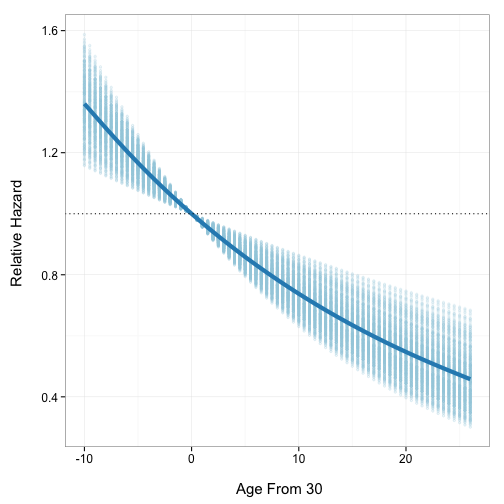
\includegraphics[width=0.7\textwidth,height=0.35\textheight]{figure/Linear4_1} 

}



\end{knitrout}

\end{figure}

A generalized additive model with integrated smoothness estimation \citep[see][]{R-mgcv} was automatically chosen to create a line that summarizes the simulations' central tendency across the range of fitted values. This can be changed in \code{simGG} with the \code{smoother} argument to any method allowed by \pkg{ggplot2}. 

If we would instead like to present the results as the percentage change in the hazard between a given age and 30, we could set the \code{coxsimLinear} \code{qi} argument to \code{'First Difference'} as in Figure \ref{Linear2}.

\begin{knitrout}
\definecolor{shadecolor}{rgb}{0.969, 0.969, 0.969}\color{fgcolor}\begin{kframe}
\begin{alltt}
\hlcomment{# Simulate relative hazards for agec}
Sim2 <- \hlfunctioncall{coxsimLinear}(M1, b = \hlstring{"agec"}, 
					 qi = \hlstring{"First Difference"},
                     Xj = \hlfunctioncall{seq}(-12, 26, by = 0.5))

\hlcomment{# Plot the results}
\hlfunctioncall{simGG}(Sim2, xlab = \hlstring{"\textbackslash{}n Age From 30"})
\end{alltt}
\end{kframe}
\end{knitrout}


\begin{figure}
	\caption{Simulated First Differences for Fitted Values of \code{agec}, Central 95\% Interval}
	\label{Linear2}
	\vspace{0.3cm}
\begin{knitrout}
\definecolor{shadecolor}{rgb}{0.969, 0.969, 0.969}\color{fgcolor}

{\centering 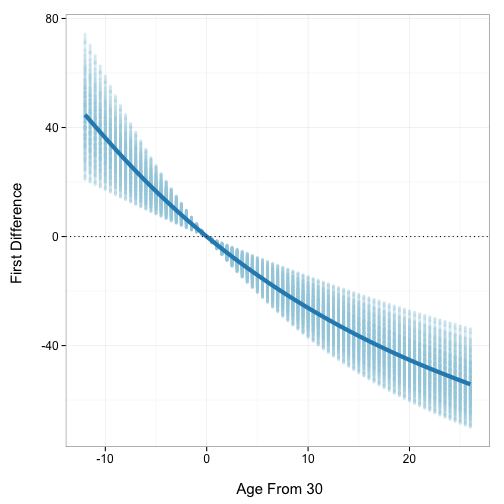
\includegraphics[width=0.7\textwidth,height=0.35\textheight]{figure/Linear5_1} 

}



\end{knitrout}

\end{figure}
\section{Conclusion}

NOTE: This vignette will be completed in coming versions of \pkg{simPH}.

% Bibliography
\bibliography{HRBibliography,HRPackages}

\end{document}
